%----------------------------------------------------------------------------------------
%	PACKAGES AND DOCUMENT CONFIGURATIONS
%----------------------------------------------------------------------------------------
\documentclass[11pt]{article}
\usepackage{amsmath} % Required for some math elements
\usepackage{hyperref} 
\usepackage{xcolor}
\usepackage{lipsum} 
\usepackage{cite}
\usepackage{graphicx} % Required for the inclusion of images
\usepackage{algorithmic}
\usepackage{array}
\usepackage{bookmark}
\usepackage{listings}
\usepackage{amssymb}
\usepackage{enumitem}
\usepackage[numbered]{mcode}
\usepackage[T1]{fontenc}
\usepackage{inconsolata}
\usepackage[margin=18mm]{geometry}
\usepackage[caption=false, font=footnotesize]{subfig}
\usepackage{fancyhdr}
\pagestyle{fancy}
\lhead{ECEN 425 Mechanical Principles 1 Submission}
\rhead{Daniel Eisen : 300447549}
\cfoot{\thepage}
\renewcommand{\headrulewidth}{0.4pt}
\renewcommand{\footrulewidth}{0.4pt}

% \usepackage[active,tightpage]{preview}
% \renewcommand{\PreviewBorder}{1in}
% \newcommand{\Newpage}{\end{preview}\begin{preview}}
  


\newlist{steps}{enumerate}{1}
\setlist[steps, 1]{label = Step \arabic*:}

\hypersetup{ %color attributes of citation, link, etc.
    colorlinks=true,
    linkcolor=blue,
    filecolor=gray,      
    urlcolor=blue,
    citecolor=blue,
}

\newcommand{\matlab}{\textsc{Matlab }} %very important and totally necessary addition
 
\newcommand\Item[1][]{%
  \ifx\relax#1\relax  \item \else \item[#1] \fi
  \abovedisplayskip=0pt\abovedisplayshortskip=0pt~\vspace*{-\baselineskip}}
%----------------------------------------------------------------------------------------
%	DOCUMENT INFORMATION
%----------------------------------------------------------------------------------------

\title{ECEN 425 \\ Mechanical Principles 1 Submission}
\author{Daniel Eisen : 300447549}
\date{\today}

\begin{document}

\maketitle
\hrule
%----------------------------------------------------------------------------------------
%	DOCUMENT CONTENT
%----------------------------------------------------------------------------------------
\begin{enumerate}
      \item $\mathrm{loss \; of \; function \; uncert:}\pm 10\%, \mathrm{max \; allow \; uncert:}\pm 30\%$
            \begin{align*}
                  n_d                                & = \frac{\mathrm{loss\ \; of \; function \; param}}{\mathrm{max \; allow \; param:}} \\
                                                     & = \frac{1/0.9}{1/1.3}=1.4\bar{4}                                                    \\
                  \mathrm{Max. \; allowable \; load} & = \frac{500}{1.44} = 346.26 \rightarrow 346N \; (3.sf)
            \end{align*}
      \item $n_d = 2.0, \; \mathrm{Nominal \; Failure} = 100N$
            \begin{align*}
                  \mathrm{Max. \; allowable \; load} & = \frac{100}{2.0} = 50N
            \end{align*}
      \item $P=8896.4N,\; S=165.5MPa,\; n_d=3.0$
            \begin{align*}
                  \sigma & = \frac{S}{n_d} = \frac{165.5}{3.0}=55.1\bar{6}            \\
                  A      & = \frac{P}{\sigma} = \frac{8896.4}{55.1\bar{6}}=161.26mm^2 \\
                  d      & = 2\sqrt{A/\pi} = 2\sqrt{161.26/\pi}=14.329083 = 14.33mm   \\
            \end{align*}
      \item $P=100N,\; r=5mm$
            \begin{align*}
                  A      & = \pi r^2 = \pi 5^2 = 78.539816          \\
                  \sigma & = \frac{P}{A}                            \\
                         & = \frac{100}{78.54} = 100/78.54=1.273237 \\
                         & = 1.27 N/mm^2 \; or \; 1.27MPa
            \end{align*}
            \newpage
      \item Used \matlab for plotting: \\
            \begin{center}
                  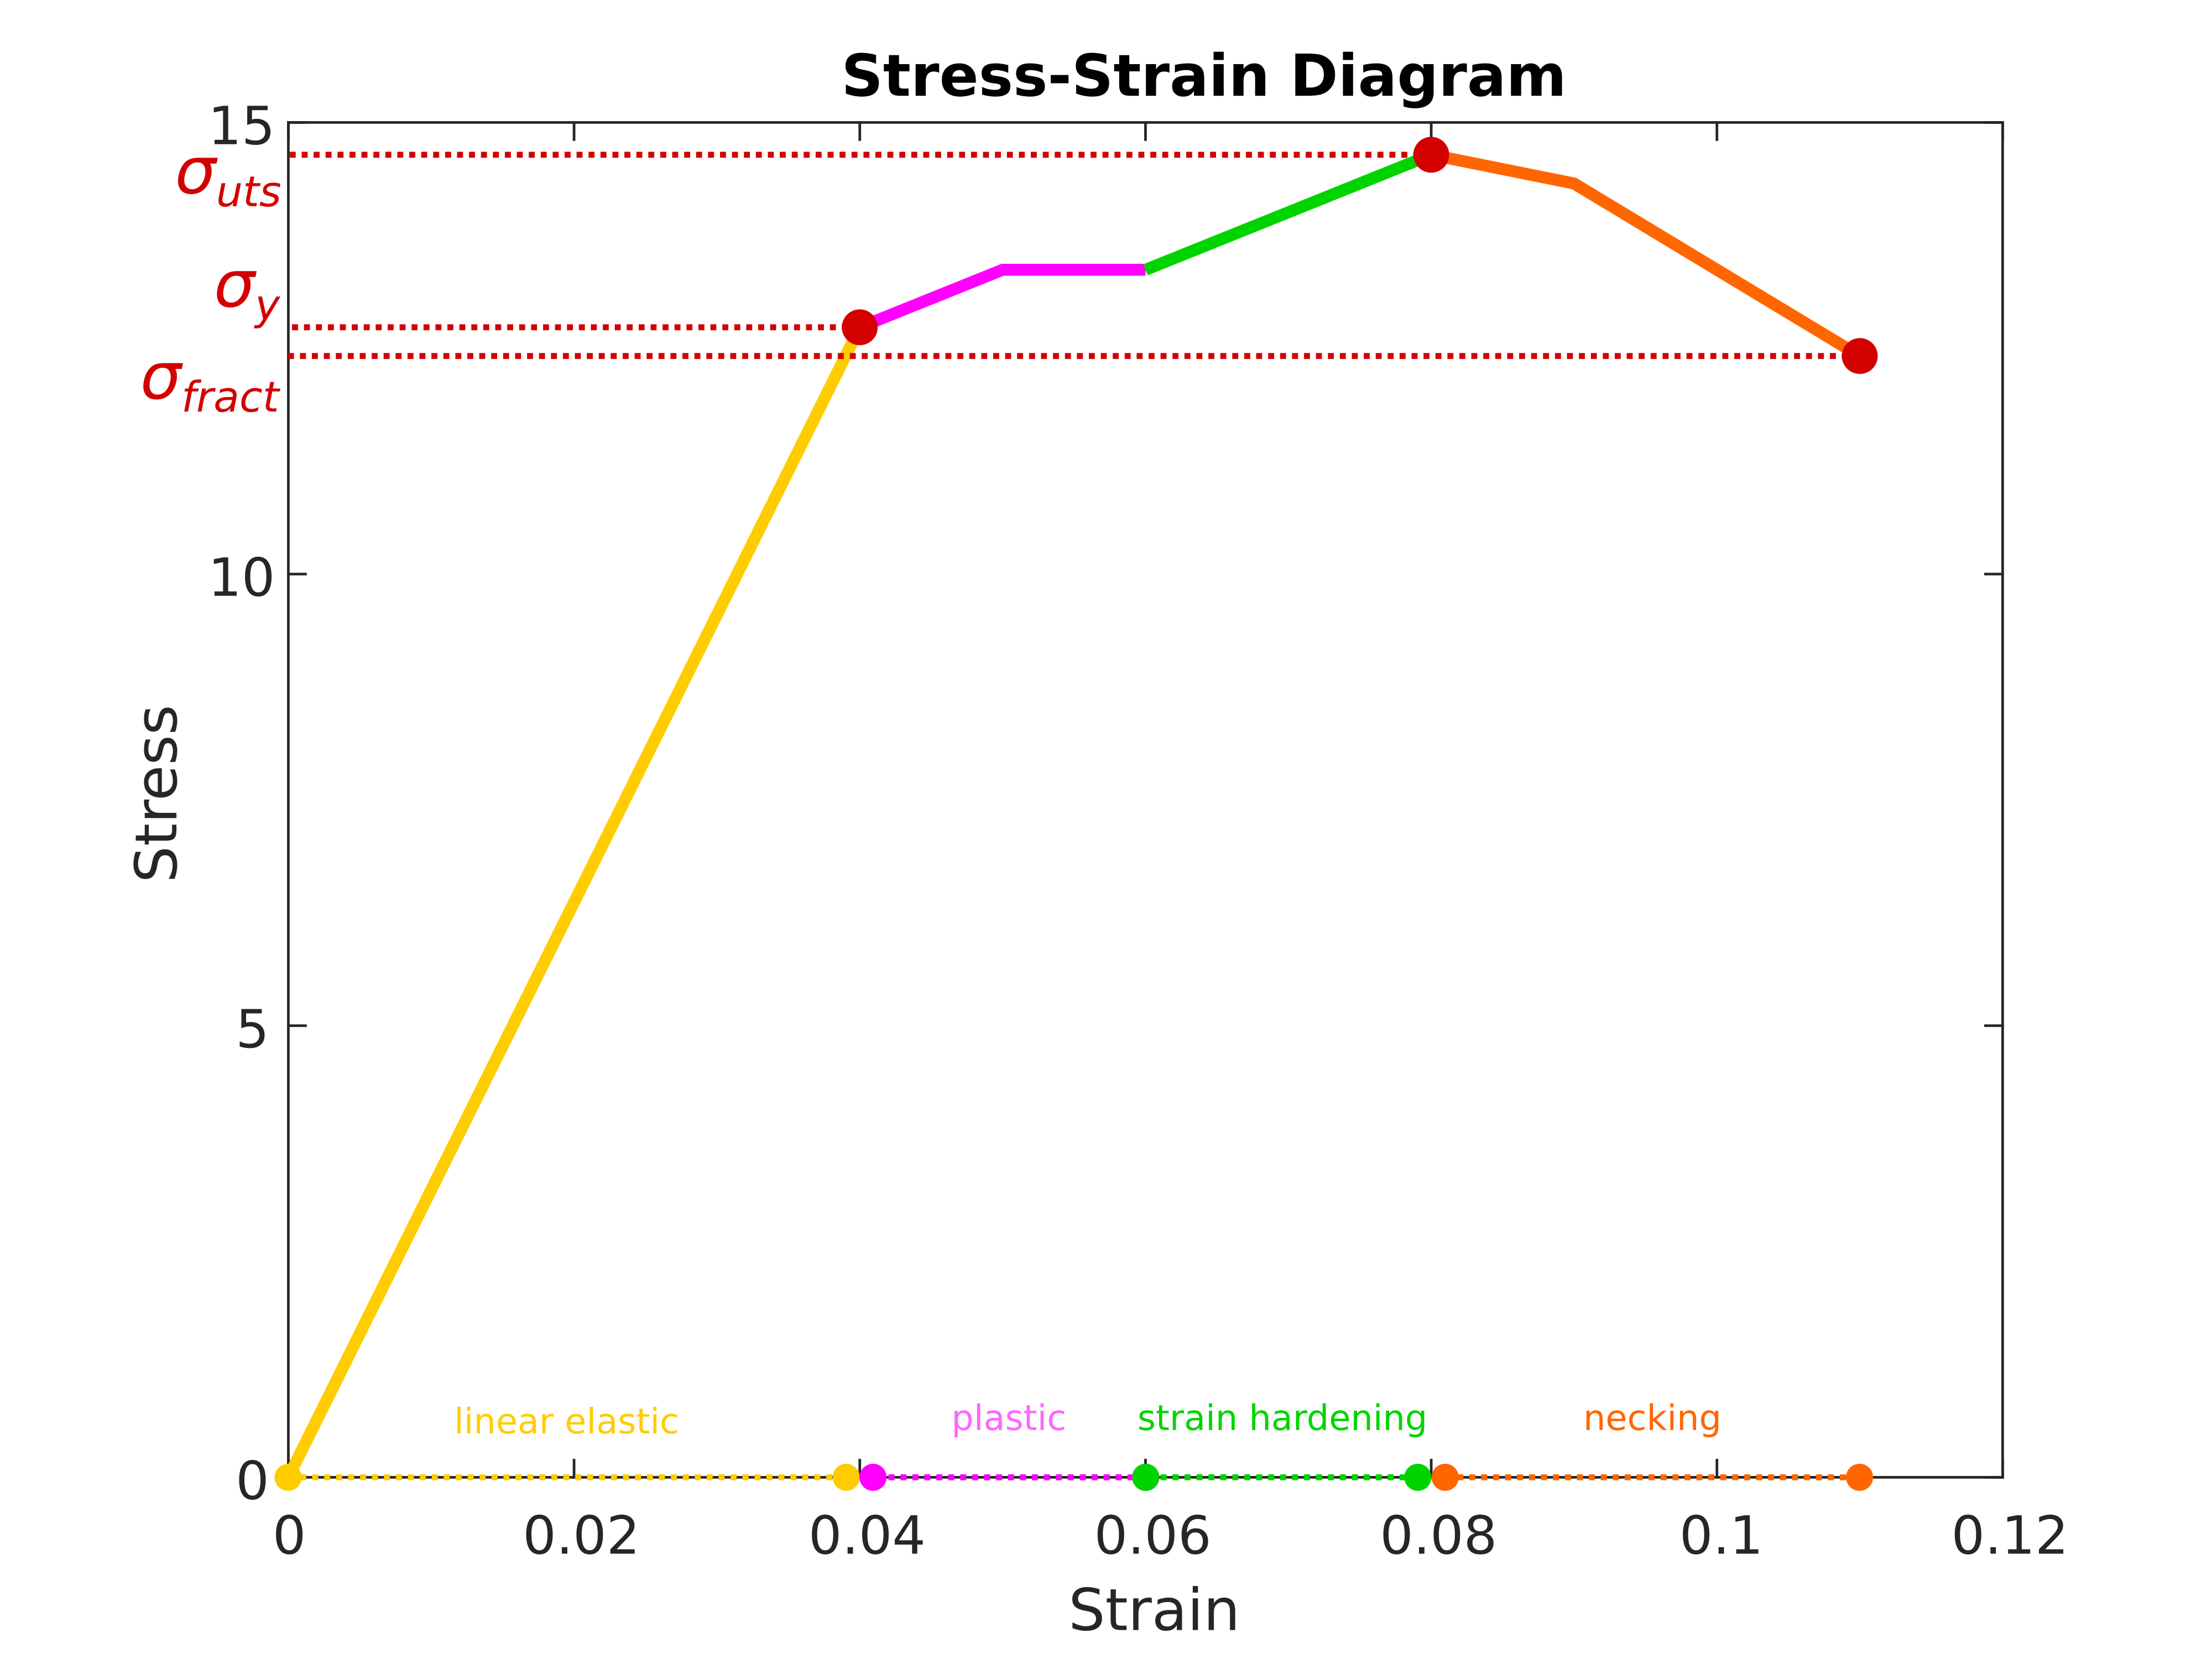
\includegraphics[width=0.5\textwidth]{q5_fig_anot.png}
            \end{center}
            \lstinputlisting{q5.m}
      \item
            \begin{enumerate}
                  \item \begin{align*}
                              E & = \frac{\Delta \sigma}{\Delta \epsilon} = \frac{12.7324}{0.04} = 318.31MPa = 0.31831GPa
                        \end{align*}
                  \item From the given examples (lecture notes), a Young's modulus of 0.31GPa puts this material more in line with the \textbf{thermoplastic} HDPE (0.8GPa) than say steel (200GPa)
                  \item Due to the assumption of \textbf{constant} diameter, this diagram (q5) has flat and decreasing slope regions where a true stress-strain diagrams would show an always upward but still slightly varying slope until fracture, i.e. because the decreasing diameter is taken into account.
            \end{enumerate}
      \item $\sigma_y = 500MPa, \; \epsilon_y = 0.02$
            \begin{align*}
                  U_r & = \frac{\sigma_y \epsilon_y}{2} = \frac{500{\cdot}0.02}{2} = 5N/mm^2
            \end{align*}
            \newpage
      \item $P = 3000kgf, \; D=10mm, \; d=5mm$
            \begin{enumerate}
                  \item \begin{align*}
                              BHN & = \frac{2P}{\pi D \left[D-\sqrt{D^2-d^2}\right]}           \\
                                  & = \frac{6000}{\pi{\cdot}10\left[10-\sqrt{10^2-5^2}\right]} \\
                                  & = 142.55
                        \end{align*}
                  \item The Brinell Hardness test as larger indenter than Rockwell so can give a better measure of average hardness across the sample.
            \end{enumerate}
      \item
            \begin{enumerate}
                  \item No, because it did not undergo any plastic deformation and is thus a brittle alloy.
                  \item No, Sea-ice collision could be characterised as a sharp impact and thus a brittle material could not sufficiently enough energy to prevent fracture. \\
                        \textit{\small "Regardless of the strength, the steel used in the hull structures of an icebreaker must be capable of resisting brittle fracture in low ambient temperatures and high loading conditions, both of which are typical for operations in ice-filled waters[1]"}\\
                        {\tiny [1] Chapter 5 Ship Design and Construction for Ice Operations. Canadian Coast Guard. Retrieved 2013-08-20.}
            \end{enumerate}
      \item $d_0=14.0mm, \; E = 111.0GPa, \; \nu = 0.349, \; P=20kN$
            \begin{align*}
                  \sigma                                 & = \frac{P}{\frac{\pi}{4}d_0^2} = \frac{20kN}{\frac{\pi}{4}14^2} = 0.12992 \frac{kN}{mm^2} \; (GPa) \\
                  \sigma = E\epsilon, \; \epsilon_{long} & = \frac{\sigma}{E} = 0.12992/111.0=0.00117                                                         \\
                  \epsilon_{lat}                         & = -\nu{\cdot}\epsilon_{long} = (-0.349)(0.00117)=-0.000408                                         \\
                  \Delta d                               & = \epsilon_{lat}{\cdot}d_0 = 14(-0.000408)=-0.005712                                               \\
                  d_f                                    & = \Delta d + d_0 = 14-0.005712=13.994288mm
            \end{align*}
      \item $l_0 = 100mm,\; l_f=100.559mm,\; d_0=10mm,\; d_f=9.980mm,\; P=50kN,\; E=114.0GPa$
            \begin{align*}
                  \epsilon_{lat}  & = -\frac{\Delta d}{d_0} =-\frac{10-9.980}{10} = -0.002                        \\
                  \epsilon_{long} & = \frac{\Delta l}{l_0} =\frac{100.559-100}{100} = 0.00559                     \\
                  \nu             & = -\frac{\epsilon_{lat}}{\epsilon_{long}} = -\frac{-0.002}{0.00559} = 0.35778
            \end{align*}
            Closest to Magnesium (0.350) but also not far from Phosphor Bronze (0.349).
      \item $P=2kN,\; A = (12mm \times 16mm) = 192mm^2$
            \begin{align*}
                  \tau_{avg} = \frac{V}{A} = \frac{2kN}{192mm^2} = 0.010417 GPa = 10417 KPa
            \end{align*}
      \item $\tau_{max} = 500KPa,\; n_d=2.0, \; V=20kN$
            \begin{align*}
                  \mathrm{max. \; load} & = 500/2 = 250KPa \\
                  A &= \frac{V}{\tau_{max}} = \frac{20kN}{0.000250GPa} = 80000mm^2
            \end{align*}
\end{enumerate}

\end{document}